\documentclass[a4paper,12pt]{article}

% Pacchetti utili
\usepackage[italian]{babel}
\usepackage[T1]{fontenc}
\usepackage[utf8]{inputenc}
\usepackage{lmodern}
\usepackage{geometry}
\usepackage{setspace}
\usepackage{graphicx}
\usepackage{titling}
\usepackage{hyperref}
\usepackage{booktabs}
\usepackage{amsmath, amssymb}
\usepackage[most]{tcolorbox}
\usepackage{tikz}
\usepackage{float}
\usetikzlibrary{arrows.meta, positioning}

\geometry{margin=2.5cm}
\onehalfspacing

\begin{document}
	
	\begin{titlepage}
		\centering
		
		% Intestazione Università
		{\scshape\LARGE Università di Pisa \par}
		\vspace{0.5cm}
		
		% Titolo corso
		{\Huge\bfseries Fondamenti di Automatica \par}
		\vspace{0.5cm}
		{\Large Anno Accademico 2025--2026 \par}
		
		\vfill
		
		% Autore
		{\Large\textbf{Pietro Bacigalupi} \par}
		\vspace{0.5cm}
		
		\vfill
		
		% Data
		{\large \today\par}
		
	\end{titlepage}
	
	\tableofcontents
	\newpage
	\section{Introduzione}
	Skippata a piè pari, se agg voglia la riscrivo
	\newpage
	\section*{Sistemi LTI}
	
	\begin{tcolorbox}[colback=white, colframe=black, arc=0mm, boxrule=0.5pt]
		Un sistema LTI (Lineare Tempo Invariante) è detto causale se l'uscita $y(t)$ per un certo $t_d$ dipende dai valori dell'ingresso $x(t)$ solo per valori $t \leq t_d$
	\end{tcolorbox}
	
	\vspace{1cm}
	
	\section{Diverse tipologie di problemi}
	
	Date tre componenti abbiamo tre tipologie diverse di problemi:
	
	\begin{enumerate}
		\item \textbf{Modellistica} (non conosciamo il sistema)
		
		\begin{center}
			\begin{tikzpicture}[node distance=2cm, auto, >=Stealth]
				\node (input) {inputs};
				\node [draw, minimum width=1cm, minimum height=0.8cm, right=of input] (sys) {?};
				\node [right=of sys] (output) {outputs};
				
				\draw [->] (input) -- (sys);
				\draw [->] (sys) -- (output);
			\end{tikzpicture}
		\end{center}
		
		\item \textbf{Simulazione} (non conosciamo l'uscita)
		
		\begin{center}
			\begin{tikzpicture}[node distance=2cm, auto, >=Stealth]
				\node (input) {inputs};
				\node [draw, minimum width=1cm, minimum height=0.8cm, right=of input] (sys) {system};
				\node [right=of sys] (output) {?};
				
				\draw [->] (input) -- (sys);
				\draw [->] (sys) -- (output);
			\end{tikzpicture}
		\end{center}
		
		\item \textbf{Controllo} (non conosciamo gli ingressi)
		
		\begin{center}
			\begin{tikzpicture}[node distance=2cm, auto, >=Stealth]
				\node (input) {?};
				\node [draw, minimum width=1cm, minimum height=0.8cm, right=of input] (sys) {system};
				\node [right=of sys] (output) {outputs};
				
				\draw [->] (input) -- (sys);
				\draw [->] (sys) -- (output);
			\end{tikzpicture}
		\end{center}
	\end{enumerate}
	\subsection{Modellistica}
	\subsubsection{Black Box}
	Si tratta di un approccio sperimentale (induttivo), in cui non conosciamo il modello ma conosciamo solo \textbf{ingressi} e \textbf{uscite}. L'approccio si compone di pochi step:
	
	\begin{itemize}
	\item Provo un numero sufficiente di ingressi.
	\item Salvo ogni ingresso in relazione alla sua uscita in una \textbf{tabella dati}.
	\item Eseguo un \textbf{fitting} sui dati nella tabella e ne ricavo un modello.
	\end{itemize}
	
	\vspace{1cm}
	
	\begin{center}
	\begin{tikzpicture}[node distance=1.5cm, auto, >=Stealth, 
		block/.style={draw, rectangle, minimum height=0.8cm, minimum width=1.5cm, align=center}]
		
		% Nodi principali (riga superiore)
		\node (in) {ingresso};
		\node [block, right=0.8cm of in] (bb) {Black Box};
		\node [block, right=1.5cm of bb] (misura) {Misura};
		\node [right=0.8cm of misura] (out) {};
		
		% Nodi inferiori
		\node [block, below=1cm of bb, xshift=1.2cm] (tabella) {Tabella Dati};
		\node [block, below=0.8cm of tabella] (fitting) {Fitting};
		\node [block, right=0.8cm of fitting] (modello) {Modello};
		
		% Collegamenti riga superiore
		\draw [->] (in) -- (bb);
		\draw [->] (bb) -- node[above] {Uscita} (misura);
		\draw [->] (misura) -- (out);
		
		% Collegamenti tratteggiati verso Tabella Dati
		% Dalla linea di ingresso
		\draw [dashed, ->] (in.east) ++(0.2,0) -- ++(0,-1.2) -| (tabella.west);
		% Dalla linea dopo Misura
		\draw [dashed, ->] (misura.east) ++(0.3,0) -- ++(0,-1.2) -| (tabella.east);
		
		% Collegamenti riga inferiore
		\draw [->] (tabella) -- (fitting);
		\draw [->] (fitting) -- (modello);
		
	\end{tikzpicture}
	\end{center}
	
	\vspace{1cm}
	
	Questo approccio funziona fin tanto che i dati in ingresso seguono circa lo stesso andamento; se di punto in bianco un ingresso si discosta da quello predetto allora il modello non sarà preciso. 
	
	Inoltre, questo approccio si adatta bene a modelli di machine learning e intelligenza artificiale, in cui si usano grandi moli di dati per addestrare e costruire un modello il più verosimile possibile. Ne consegue che questo approccio ha molto senso in sistemi troppo complessi.
	\subsubsection{White Box}
	\subsubsection{Gray Box}
	\subsubsection{Approccio Pragmatico}
	\subsubsection{Macchine a Stati}
	\begin{tcolorbox}
		Si definisce \textbf{segnale di riferimento}, \emph{set point} $h^{\circ}(t) = \bar{h}$ l'oggetto che desidero in uscita ($h^{\circ}$ è $h$ output)
	\end{tcolorbox}
	Esiste una relazione tra lo stato $x$ e la sua derivata $\dot{x}$
	\begin{center}
		\begin{tikzpicture}[
			% Definizione dello stile per i blocchi
			block/.style={draw, rectangle, minimum height=1.5cm, minimum width=0.8cm, align=center, line width=0.6pt},
			% Definizione dello stile per le frecce
			arrow/.style={->, >=Stealth, line width=0.6pt}
			]
			
			% --- PRIMO GRAFICO (Sinistra) ---
			\node (in1) {};
			\node [block, right=1.5cm of in1] (int1) {\huge $\int$};
			\node (out1) [right=1.5cm of int1] {};
			
			\draw [arrow] (in1) -- node[above, pos=0.5] {$\dot{x}$} (int1);
			\draw [arrow] (int1) -- node[above, pos=0.5] {$x$} (out1);
			
			% --- SECONDO GRAFICO (Destra) ---
			% Posizionato a destra del primo
			\node (in2) [right=3.5cm of out1] {};
			\node [block, right=1.5cm of in2] (int2) {\huge $\frac{1}{s}$};
			\node (out2) [right=1.5cm of int2] {};
			
			\draw [arrow] (in2) -- node[above, pos=0.5] {$\dot{x}$} (int2);
			\draw [arrow] (int2) -- node[above, pos=0.5] {$x$} (out2);
			
		\end{tikzpicture}
	\end{center}
	Ci sono vari esempi che poi magari scriverò...
	\newpage 
	\section{Sistemi lineari e Tempo Invarianti (LTI)}
	Tutti i sistemi LTI hanno le seguenti proprietà:
	\begin{itemize}
		\item \textbf{Omogeneità}: Se si scala l'ingresso $u(t)$ anche l'uscita $y(t)$ verrà scalata:
		\begin{equation*}
			a \cdot u(t) = a \cdot y(t)
		\end{equation*}
		\item \textbf{Sovrapposizione degli effetti}: Se un modello di sistema ha risposte $y_1(t), y_2(t)$ a due ingressi qualsiasi $x_1(t), x_2(t)$, la risposta del sistema alla combinazione lineare di questi ingressi:
		\begin{equation*}
			a_1x_1(t) + a_2x_2(t)
		\end{equation*}
		è data dalla combinazione lineare delle risposte individuali:
		\begin{equation*}
			a_1y_1(t) + a_2y_2(t)
		\end{equation*}
		\item \textbf{Invarianza nel tempo}
		Il sistema si comporta allo stesso modo indipendentemente da quando avviene l'azione, non vi è una dipendenza esplicita dal tempo. Un ingresso $x(t - \tau)$ produce un'uscita $y(t - \tau)$
	\end{itemize}
	\subsection{Equazioni differenziali lineari}
	La rappresentazione standard per rappresentare la dinamica di un sistema è la seguente:
	\begin{equation}
		\begin{cases}
			\dot{x} = Ax + Bu, &x: \text{stato}, u: \text{ingresso}\\
			y = Cx + Du, &y: \text{uscita}
		\end{cases}
	\end{equation}
	\begin{equation*}
		u \in \mathbb{R}^r, x \in \mathbb{R}^n, y \in \mathbb{R}^m, A \in \mathbb{R}^{n \times n}, B \in \mathbb{R}^{n \times r}, C \in \mathbb{R}^{m \times n}, D \in \mathbb{R}^{m \times r}
	\end{equation*}
	Possiamo ricavare dalla prima equazione $x(t)$ ossia il \textbf{movimento dello stato del sistema}. La seconda equazione $y(t)$ è detta \textbf{movimento dell'uscita del sistema}
	\paragraph{Equilibrio di un sistema}
	
	Dato il sistema $\dot{x} = f(x, u)$ (forma standard dell'equazione di stato) e dato un ingresso costante $u(t) = \bar{u}$:
	
	\begin{tcolorbox}[colback=white, colframe=black, arc=0mm, boxrule=0.5pt]
		Uno stato $\bar{x}$ si dice in \textbf{equilibrio} se soddisfa la relazione:
		\[ 0 = f(\bar{x}, \bar{u}) \]
	\end{tcolorbox}
	
	In questa condizione, il sistema \textbf{non si muove} da $\bar{x}$. Se il sistema si trova in $\bar{x}$ all'istante $t_0$, vi rimarrà per ogni $t > t_0$ a patto che l'ingresso non vari.
	Definiamo due nuove variabili che rappresentano la \textbf{variazione di equilibrio} 
	\begin{align*}
		\varDelta{x} = x - \bar{x} \\
		\varDelta{u} = u - \bar{u} 
	\end{align*}
	\begin{figure}[H] % Ambiente figure
		\centering
		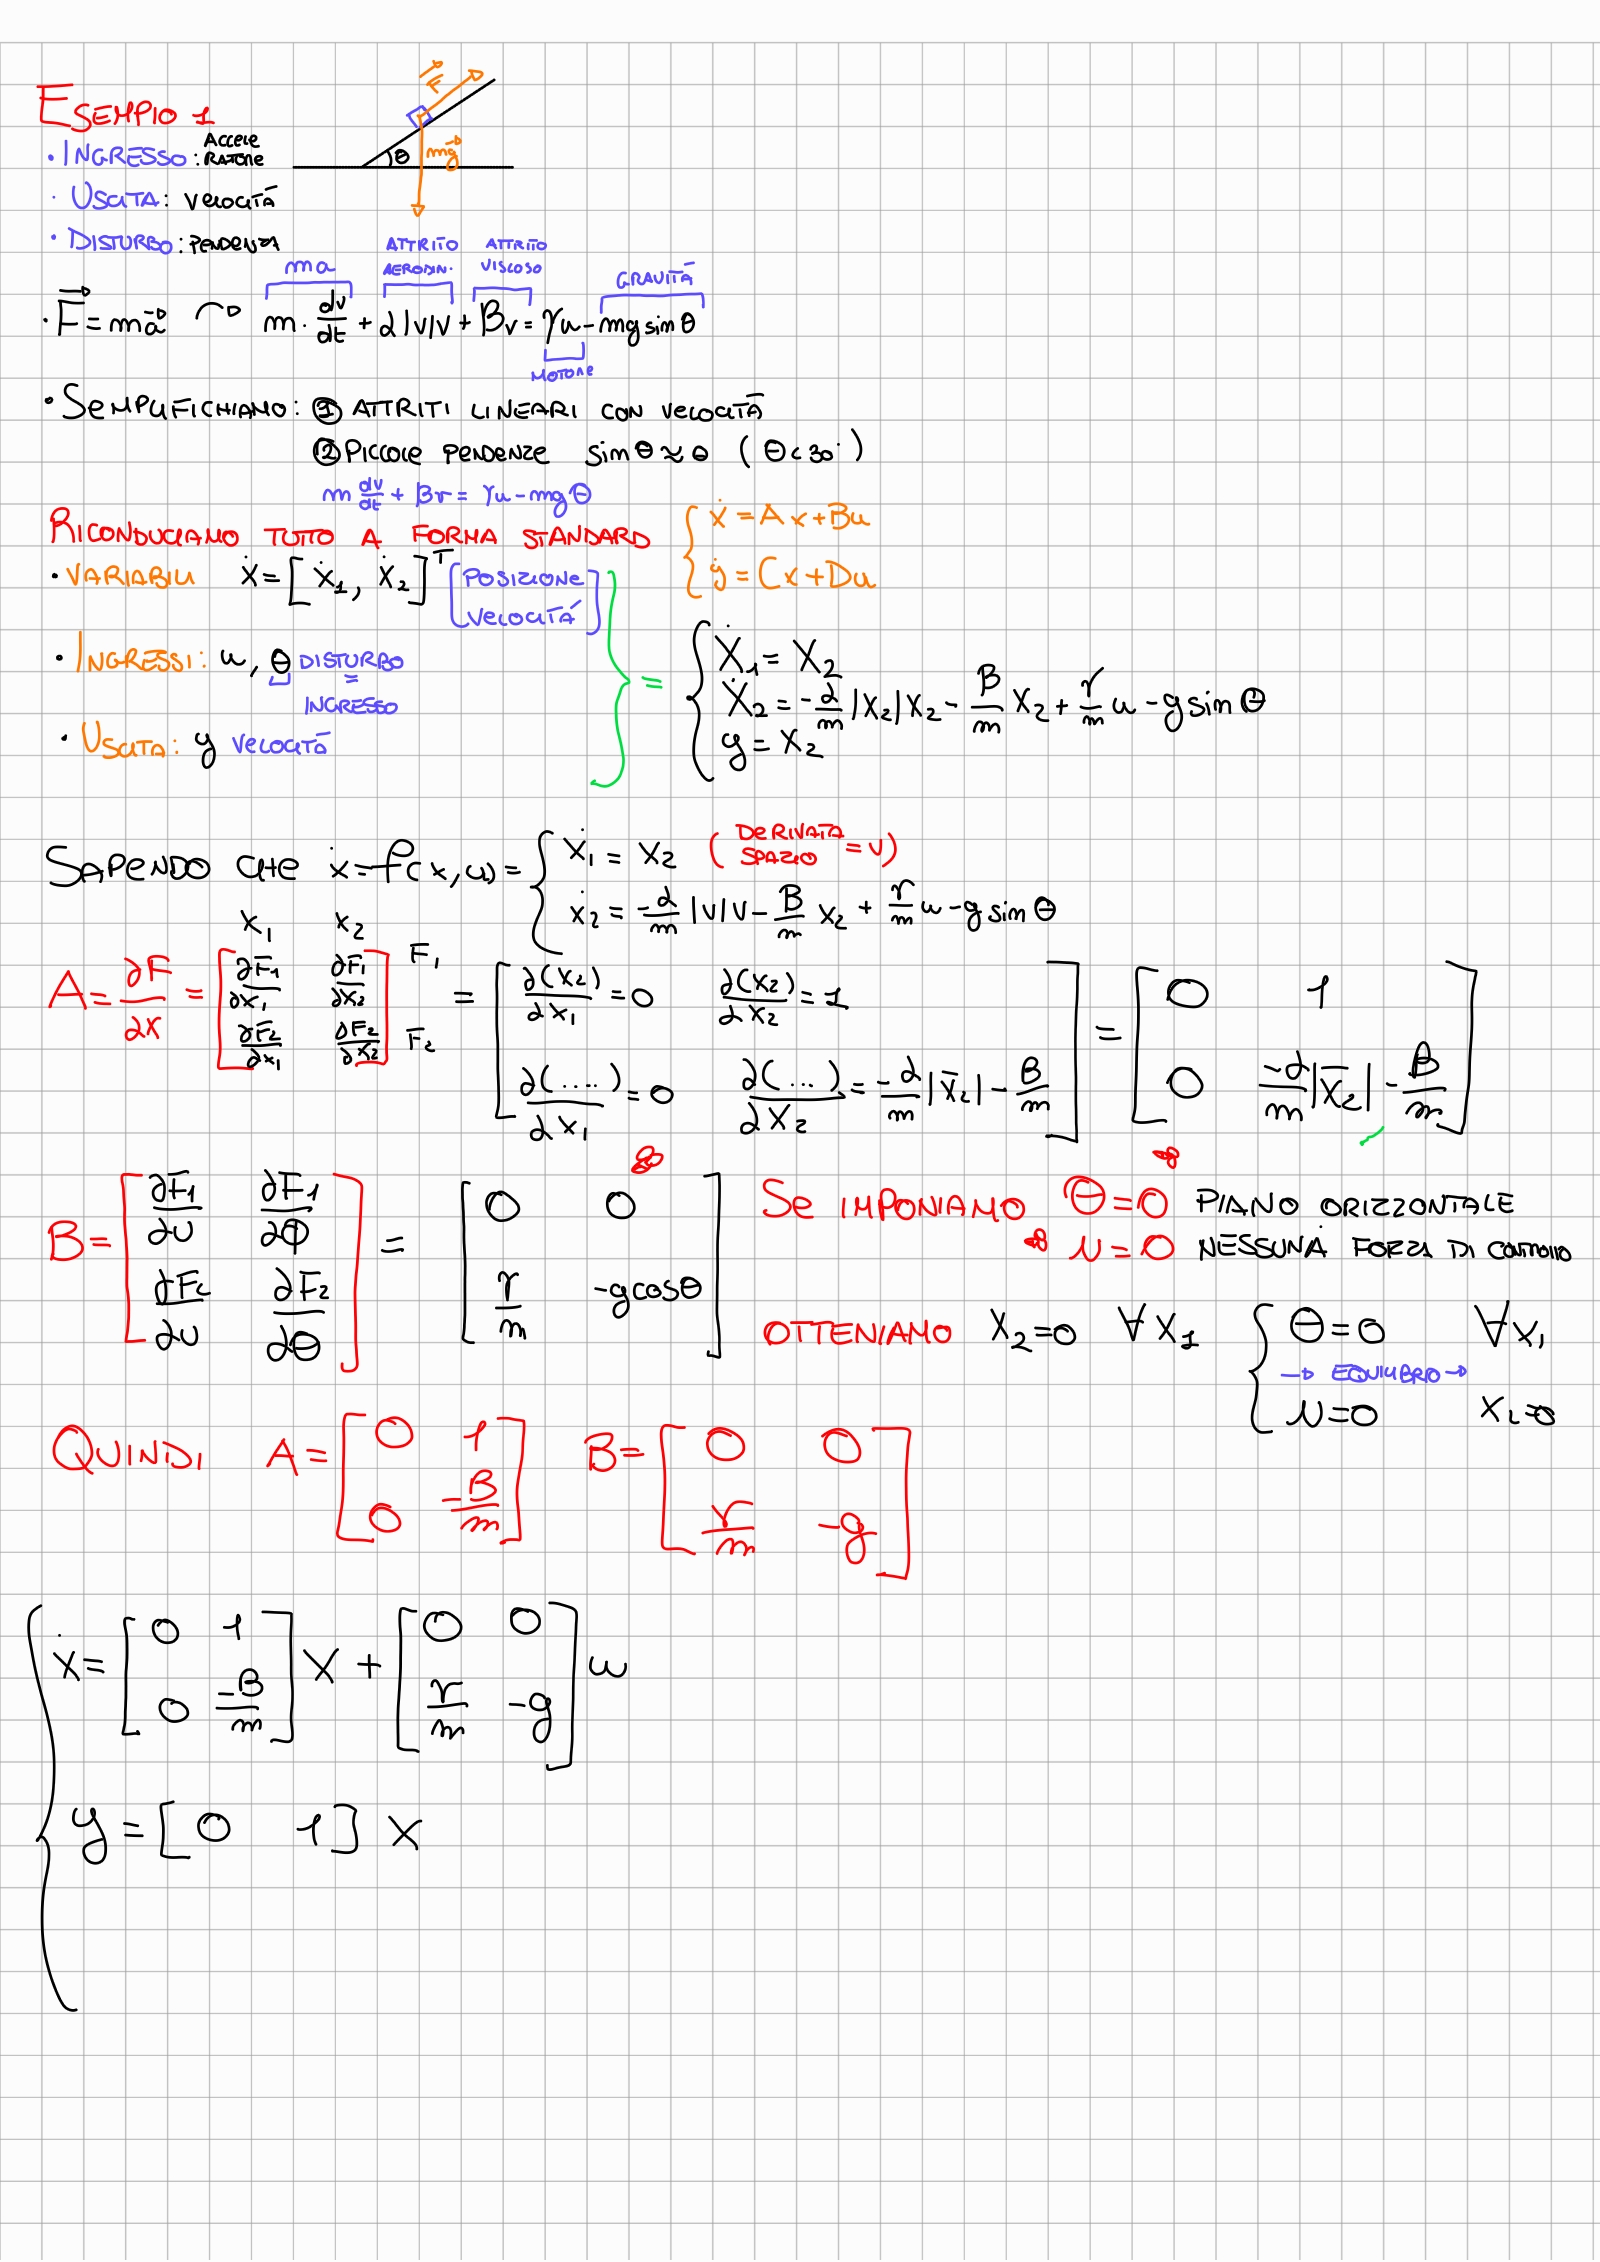
\includegraphics[width=\textwidth]{figura_1.jpg} % Inserimento
		\caption{Didascalia della figura}
		\label{fig:label_immagine}
	\end{figure}
	
	\section{Stabilità (secondo Lyapunov)}
	La stabilità considera le conseguenze sul movimento del sistema di un'incertezza sul valore iniziale dello stato (Ipotesi ingressi fissi e noti).
	"Piccole" perturbazioni dello stato iniziale rispetto ad un valore di riferimento provocano sole "piccole" perturbazioni nel movimento dello stato, eventualmente destinate ad annullarsi per "tempi lunghi".
	
	\subsection{Stabilità dell'equilibrio}
	Scelgo un ingresso costante $u(t) = \bar{u}$ corrispondente allo stato di equilibrio $\bar{x}$.
	
	Consideriamo un \textbf{Movimento Perturbato} ottenuto da $u(t) = \bar{u}$ ma a partire da $x_0$ (diverso da $\bar{x}$). Allora definiremo:
	
	Uno stato di equilibrio $\bar{x}$ è stabile, se per ogni $\varepsilon > 0$ esiste $\delta > 0$ tale che per tutti gli $x_0$ che soddisfano 
	\begin{align*}
		\|x_0 - \bar{x}\| \leq \delta 
	\end{align*}
	Si ha $\|x(t) - \bar{x}\| \leq \varepsilon, t \geq 0$
	
	\subsection{Asintotica stabilità}
	UNo stato di equilibrio $\bar{x}$ è asintoticamente stabile, se per ogni $\varepsilon > 0$ esiste $\delta > 0$ tale che per tutti gli $x_0$ che soddisfano
	\begin{align*}
		\|x_0 - \bar{x}\| \leq \delta 
	\end{align*}
	Si ha che
	\begin{align*}
		\|x(t) - \bar{x}\| \leq \varepsilon, t \geq 0
	\end{align*}
	E inoltre abbiamo che:
	\begin{align*}
		\lim\limits_{t \rightarrow \infty} \|x(t) - \bar{x}\| = 0
	\end{align*}
	Il seguente grafico mostra i vari tipi di stabilità in uno stato.
	
		\begin{tikzpicture}[scale=0.5]
			
			% Legenda a sinistra
			\node[align=left, anchor=north east] at (-0.5, 4.5) {
				\textbf{A} è stabile \\ 
				\textbf{B} è asintoticamente stabile \\ 
				\textbf{C} è instabile
			};
			
			% Assi cartesiani
			\draw[->, thick] (0,0) -- (6,0) node[below] {$X$};
			\draw[->, thick] (0,0) -- (0,5) node[below right] {$E_{\text{pot}}$};
			
			% Curva dell'energia potenziale
			\draw[very thick] (0.2, 2.5) -- (1.4, 2.5) 
			.. controls (1.8, 2.5) and (1.8, 0.5) .. (2.4, 0.5) 
			.. controls (3.0, 0.5) and (3.3, 4.2) .. (4.0, 4.2) 
			.. controls (4.6, 4.2) and (4.8, 1.5) .. (5.1, 1.0);
			
			% Pallina A
			\filldraw[fill=lightgray, draw=black, thick] (0.8, 2.65) circle (0.15) node[above=3pt, text=black] {\textsf{A}};
			
			% Pallina B
			\filldraw[fill=lightgray, draw=black, thick] (2.4, 0.65) circle (0.15) node[above=3pt, text=black] {\textsf{B}};
			
			% Pallina C
			\filldraw[fill=lightgray, draw=black, thick] (4.0, 4.35) circle (0.15) node[above=3pt, text=black] {\textsf{C}};
			
		\end{tikzpicture}
	
	\section{Formula di Lagrange}
	Lagrange insieme a Lyapunov rappresenta un punto cardine per i controllisti.
	\begin{gather*}
		\left\{
		\begin{aligned}
			\dot{x} &= Ax + Bu, && \quad x : \text{stato}, \ u : \text{ingresso} \\
			y &= Cx + Du, && \quad y : \text{uscita}
		\end{aligned}
		\right. \\[15pt]
		u \in \mathbb{R}^r, \qquad x \in \mathbb{R}^n, \qquad y \in \mathbb{R}^m, \\
		A \in \mathbb{R}^{n \times n}, \qquad B \in \mathbb{R}^{n \times r}, \qquad C \in \mathbb{R}^{m \times n}, \qquad D \in \mathbb{R}^{m \times r}
	\end{gather*}
	
	Per sistemi LTI possiamo calcolare in forma chiusa la \textbf{funzione di transizione dello stato}, ovvero la soluzione:
	\[
	\begin{cases}
		x(t) = \phi(t, t_0, x(t_0), u(t)) \\
		y(t) = \gamma(t, t_0, x(t_0), u(t))
	\end{cases}
	\]
	\subsection{Equazioni differenziali lineari}
	\subsubsection{Soluzioni esplicite}
	Una equazione differenziale scalare e omogenea:
	\[
	\begin{cases}
		\dot{x}(t) = a \cdot x(t) \\
		x(t_0 = 0) = x_0
	\end{cases}
	\]
	Ha una soluzione del tipo $x(t) = x_0e^{at}$.
	Il comportamento dipende dal segno e dal valore di $a$ o della sua parte reale
	\[
		e^{at} = e^{(x+jy)t} = e^xt(\cos(y) + j\sin(y))
	\]
	Sviluppando in serie la funzione esponenziale
	\[
	e^{at} = \sum_{i = 0}^{\infty} a^i\frac{t^i}{i!} = at + a^2\frac{t^2}{2!} + \dots + a^r \frac{t^r}{r!} + \dots \quad a \in \mathbb{R}
	\]
	\subsubsection{Soluzioni vettoriali}
	Consideriamo il caso vettoriale omogeneo (sistema LTI con $u(t) = 0$).
	
	\[
	\begin{cases}
		\dot{x}(t) = A \cdot x(t) \\
		x(t_0 = 0) = x_0
	\end{cases}
	\]
	La soluzione dell'equazione vettoriale è simile a quella vista prima.
	\[
	 x(t) = x_0e^{At}
	\]
	dove 
	\[
	e^{At} = \sum_{i = 0}^{\infty} A^i\frac{t^i}{i!} = I + At + A^2\frac{t^2}{2!} + \dots + A^r \frac{t^r}{r!} + \dots 
	\]
	è detta esponenziale della matrice $A$
	\subsubsection{Matrice di transizione}
	$e^{At}$ è chiamata matrice di transizione perché determina in assenza di ingresso ($u(t) = 0$) il moto libero del sistema
	\[
		x(t) = \phi(t, t_0, x(t_0), u = 0) = e^{A(t-t_0)}x(t_0)
	\]
	
	Allora definiamo matrice di transizione dello stato $\varPhi(t, t_0)$ la soluzione dell'equazione differenziale matriciale (caso non stazionario).
	\[
		\dot{X} = A(t)X(t); \quad X(t_0) = X_0
	\]
	
	\section{Evoluzione dello stato per sistemi LTI}
	\subsection{Formula di Lagrange}
	Sia dato $\bar{x} = Ax + Bu \quad x(t_0 = 0) = x_0$
	
	Si dimostra che la soluzione dell'equazione differenziale, ovvero il movimento dello stato in corrispondenza di un certo ingresso $u(t) \neq 0$ è data dalla \textbf{Formula di Lagrange}:
	\[
	\dot{x} = Ax + Bu \Rightarrow x(t) = \underset{\textcolor{green!60!black}{\text{risposta libera}}}{e^{At}x_0} + \underset{\textcolor{green!60!black}{\text{risposta forzata}}}{\int_{t_0}^{t} e^{A(t-\tau)}Bu(\tau)d\tau},
	\]
	
	Nota bene in un sistema più generico con $t_0 \neq 0$ abbiamo:
	
	\[
	x(t) = \underset{\textcolor{green!60!black}{\text{risposta libera}}}{e^{A(t-t_0)}x_0} + \underset{\textcolor{green!60!black}{\text{risposta forzata}}}{\int_{t_0}^{t} e^{A(t-\tau)}Bu(\tau)d\tau}, \qquad t \geq t_0, \ x_0 = x(t_0)
	\]
	\begin{itemize}
		\item \textbf{Risposta libera} $\varphi(t, t_0, x_0, u(t) = 0)$:
		
		Il \textbf{movimento libero} (dello stato o dell'uscita) è l'evoluzione del sistema dovuta esclusivamente allo stato iniziale. In altre parole, è il comportamento che il sistema avrebbe se non vi fosse applicato alcun ingresso esterno $(u(t) = 0)$. 
		\[
		x_l(t) = e^{A(t-t_0)}x_0 \quad y_l(t) = Ce^{A(t-t_0)}x_0
		\]
		
		\item \textbf{Risposta forzata} $\varphi(t, t_0, x(t_0) = 0, u(t))$:
		
		Il \textbf{movimento forzato} (dello stato o dell'uscita) è l'evoluzione del sistema causata esclusivamente dai segnali di ingresso. In altre parole, è la risposta che il sistema avrebbe se partisse da una condizione di riposo assoluto, ovvero con stato iniziale nullo $x_0 = 0$.
		\[
			x_f(t) = \int_{t_0}^{t} e^{A(t-\tau)}Bu(\tau)d\tau \quad y_f(t) = C \int_{t_0}^{t} e^{A(t-\tau)}Bu(\tau)d\tau + Du(t)
		\]
	\end{itemize}
	Al \textbf{Movimento dello stato} $x(t)$ dal sistema LTI ricaviamo anche il corrispondente \textbf{Movimento dell'uscita}:
	\[
	y(t) = Cx(t) + Du(t)
	\]
	
	\subsection{Principio di sovrapposizione degli effetti}
	
	Il \textbf{principio di sovrapposizione degli effetti} è un concetto di fondamentale importanza nello studio dei sistemi. Esso ci permette di calcolare il comportamento complessivo del sistema (generato da più cause, come le condizioni iniziali e i segnali di ingresso) calcolandolo semplicemente come la somma lineare dei singoli effetti provocati da ciascuna di queste cause presa singolarmente.
	
	Per descrivere matematicamente il legame generale tra le cause e gli effetti in un sistema dinamico, si utilizza un'equazione differenziale che in forma implicita si presenta così:
	
	\[
	F(y(t), y^{(1)}(t), \dots, y^{(n)}(t), u(t), u^{(1)}(t), \dots, u^{(p)}(t), t) = 0
	\]
	
	Esplicitando questa equazione rispetto alla derivata di ordine massimo dell'uscita, otteniamo la forma:
	
	\[
	y^{(n)}(t) = \hat{F}(y(t), y^{(1)}(t), \dots, y^{(n-1)}(t), u(t), u^{(1)}(t), \dots, u^{(p)}(t), t)
	\]
	
	All'interno di queste equazioni possiamo riconoscere chiaramente le componenti fondamentali del sistema:
	\begin{itemize}
		\item Le variabili $y(t), y^{(1)}(t), \dots, y^{(n)}(t)$ identificano l'\textbf{uscita} del sistema e le sue derivate nel tempo. Esse rappresentano gli \textit{effetti} che osserviamo.
		\item Le variabili $u(t), u^{(1)}(t), \dots, u^{(p)}(t)$ identificano l'\textbf{ingresso} applicato al sistema e le sue derivate nel tempo. Esse rappresentano le \textit{cause} che ne influenzano il comportamento.
	\end{itemize}
	\subsection{Rappresentazioni equivalenti}
	
	Partendo dall'equazione differenziale generale di ordine $n$, possiamo sempre ricondurci a un sistema equivalente composto da $n$ equazioni differenziali del primo ordine. Definendo il vettore di stato $x(t)$, otteniamo la rappresentazione in spazio di stato:
	
	\[
	\dot{x}(t) = 
	\begin{bmatrix} 
		\dot{x}_1(t) \\ 
		\vdots \\ 
		\dot{x}_n(t) 
	\end{bmatrix} 
	= 
	\begin{bmatrix} 
		f_1(\dots) \\ 
		\vdots \\ 
		f_n(\dots) 
	\end{bmatrix} 
	\underset{\text{se lineare}}{=} Ax + Bu
	\]
	
	\textbf{Nota Bene sui parametri:}
	\begin{itemize}
		\item $n$ rappresenta l'ordine del sistema, ovvero il grado massimo di derivazione dell'uscita $y(t)$.
		\item $p$ rappresenta il grado massimo di derivazione dell'ingresso $u(t)$. Ci indica fino a quale derivata (velocità, accelerazione, ecc. del segnale) l'ingresso influisce sul comportamento del sistema.
	\end{itemize}
	
	\subsubsection{Rappresentazioni equivalenti per $p = 0$}
	
	Nel caso particolare in cui il sistema non dipenda dalle derivate dell'ingresso (ovvero $p = 0$, il sistema reagisce solo al valore istantaneo di $u(t)$), una scelta naturale e molto comune per definire il vettore di stato è quella di utilizzare le \textit{variabili di fase}. Si sceglie cioè la prima variabile di stato pari all'uscita ($x_1 = y$) e le successive pari alle sue derivate:
	
	\[
	x = 
	\begin{bmatrix} 
		x_1 \\ 
		\vdots \\ 
		x_n 
	\end{bmatrix} 
	= 
	\begin{bmatrix} 
		y \\ 
		\vdots \\ 
		y^{(n-1)} 
	\end{bmatrix} 
	\qquad 
	\dot{x} = 
	\begin{bmatrix} 
		\dot{x}_1(t) \\ 
		\vdots \\ 
		\dot{x}_n(t) 
	\end{bmatrix} 
	= 
	\begin{bmatrix} 
		f_1(\dots) \\ 
		\vdots \\ 
		f_n(\dots) 
	\end{bmatrix}
	\]
	
	Poiché ogni variabile di stato è la derivata della precedente (es. $\dot{x}_1 = x_2$, $\dot{x}_2 = x_3$, ecc.), il sistema si semplifica notevolmente assumendo questa forma a cascata:
	
	\[
	\dot{x} = 
	\begin{bmatrix} 
		\dot{x}_1 \\ 
		\vdots \\ 
		\dot{x}_n 
	\end{bmatrix} 
	= 
	\begin{bmatrix} 
		x_2 \\ 
		\vdots \\ 
		x_n \\ 
		\hat{F}([y, \dots, y^{(n-1)}], u, t) 
	\end{bmatrix} 
	= 
	\begin{bmatrix} 
		x_2 \\ 
		\vdots \\ 
		x_n \\ 
		\hat{F}(x, u, t) 
	\end{bmatrix} 
	= \bar{f}(x, u, t)
	\]
	
	Inoltre, se restringiamo il campo ai soli \textbf{sistemi lineari}, la funzione esplicita $\hat{F}$ (che modella la dinamica dell'ultima derivata) diventa una semplice combinazione lineare. L'equazione di ordine $n$ si esprime quindi come:
	
	\[
	y^{(n)} = \sum_{i=0}^{n-1} -\alpha_i(t)y^{(i)}(t) + u(t) \qquad (p = 0)
	\]
	
	\[
	\begin{cases}
		\dot{x} = 
		\begin{bmatrix} 
			0 & 1 & 0 & \dots & 0 \\ 
			0 & 0 & 1 & \dots & 0 \\ 
			\vdots & \vdots & \vdots & \ddots & 0 \\ 
			0 & 0 & 0 & \dots & 1 \\ 
			-\alpha_0 & -\alpha_1 & \dots & -\alpha_{n-2} & -\alpha_{n-1} 
		\end{bmatrix} 
		x + 
		\begin{bmatrix} 
			0 \\ 
			0 \\ 
			\vdots \\ 
			0 \\ 
			1 
		\end{bmatrix} 
		u, \qquad p = 0 
		\\
		\\
		y = 
		\begin{bmatrix} 
			1 & 0 & \dots & 0 
		\end{bmatrix} 
		x + [0] u
	\end{cases}
	\]
	
	Quest'ultima matrice è detta \textbf{matrice in forma compagna orizzontale inferiore}.
	
	\vspace{0.5cm}
	
	\subsubsection*{A cosa serve e come si usa (Esempio Pratico)}
	
	La forma compagna è uno strumento potentissimo perché ci permette di passare da un'equazione differenziale (che descrive il sistema) alla sua rappresentazione matriciale in Spazio di Stato in modo quasi automatico, senza dover fare calcoli complessi. Basta "leggere" i coefficienti dell'equazione e scriverli nell'ultima riga della matrice, cambiati di segno.
	
	\textbf{Esempio:}
	Immaginiamo di avere un sistema meccanico descritto dalla seguente equazione differenziale del terzo ordine ($n=3$):
	\[
	\dddot{y}(t) + 4\ddot{y}(t) + 5\dot{y}(t) + 2y(t) = u(t)
	\]
	
	Per prima cosa, isoliamo la derivata di ordine massimo a sinistra (come abbiamo visto nella forma $\hat{F}$):
	\[
	\dddot{y}(t) = -2y(t) - 5\dot{y}(t) - 4\ddot{y}(t) + u(t)
	\]
	
	I coefficienti originali dell'equazione sono $\alpha_0 = 2$, $\alpha_1 = 5$, e $\alpha_2 = 4$. Sfruttando la struttura predefinita della forma compagna, possiamo scrivere immediatamente il nostro sistema:
	
	\[
	\begin{cases}
		\dot{x} = 
		\begin{bmatrix} 
			0 & 1 & 0 \\ 
			0 & 0 & 1 \\ 
			-2 & -5 & -4 
		\end{bmatrix} 
		x + 
		\begin{bmatrix} 
			0 \\ 
			0 \\ 
			1 
		\end{bmatrix} 
		u 
		\\
		\\
		y = 
		\begin{bmatrix} 
			1 & 0 & 0 
		\end{bmatrix} 
		x
	\end{cases}
	\]
	
	\textbf{Vantaggio teorico:} Oltre alla facilità di scrittura, questa forma è molto amata nella Teoria dei Controlli. Il calcolo degli autovalori (fondamentali per la stabilità) è immediato: il polinomio caratteristico di questa matrice coincide esattamente con i coefficienti dell'equazione differenziale di partenza ($\lambda^3 + 4\lambda^2 + 5\lambda + 2 = 0$).
	\subsubsection{Rappresentazioni equivalenti per $0 < p < n$}
	
	Nel caso più generale in cui il sistema dipenda anche dalle derivate dell'ingresso ($0 < p < n$), l'equazione differenziale per un sistema lineare assume questa forma:
	
	\[
	y^{(n)} = \sum_{i=0}^{n-1} -\alpha_i(t)y^{(i)}(t) + \sum_{j=0}^{p} \beta_j u^{(j)}(t) \qquad (0 < p < n)
	\]
	
	Per ricondurre questo sistema alla forma in spazio di stato, evitando di inserire le derivate dell'ingresso nelle variabili di stato, introduciamo una \textbf{variabile ausiliaria} $z(t)$. Definiamo un'equazione differenziale fittizia in cui la variabile $z(t)$ è eccitata solo dall'ingresso puro $u(t)$, mantenendo la stessa dinamica interna (stessi coefficienti $\alpha_i$):
	
	\[
	z^{(n)} = \sum_{i=0}^{n-1} -\alpha_i(t)z^{(i)}(t) + u(t) \quad \longleftrightarrow \quad x = \begin{bmatrix} z \\ \dot{z} \\ \vdots \\ z^{(n-1)} \end{bmatrix}
	\]
	
	Questa equazione ausiliaria descrive la risposta del sistema al semplice ingresso $u(t)$. Il nuovo vettore di stato $x$ viene quindi definito utilizzando $z$ e le sue derivate, permettendoci di ricadere nella comodità del caso $p=0$ visto in precedenza.
	
	A questo punto, sfruttiamo il \textbf{principio di sovrapposizione degli effetti}. Poiché il sistema è lineare, se l'ingresso reale è una combinazione lineare di $u(t)$ e delle sue derivate (pesate dai coefficienti $\beta_j$), allora l'uscita reale $y(t)$ sarà l'esatta medesima combinazione lineare della risposta ausiliaria $z(t)$ e delle sue derivate.
	
	Abbiamo quindi ottenuto che l'uscita $y(t)$ è semplicemente:
	
	\[
	y(t) = \sum_{j=0}^{p} \beta_j z^{(j)}(t)
	\]
	
	Possiamo quindi scrivere il sistema completo in forma matriciale per $0 < p < n$:
	
	\[
	\begin{cases}
		\dot{x} = 
		\left[
		\begin{array}{c|cccc} 
			0 & 1 & 0 & \dots & 0 \\ 
			0 & 0 & 1 & \dots & 0 \\ 
			\vdots & \vdots & \vdots & \ddots & \vdots \\ 
			0 & 0 & 0 & \dots & 1 \\ 
			\hline
			-\alpha_0 & -\alpha_1 & \dots & -\alpha_{n-2} & -\alpha_{n-1} 
		\end{array}
		\right] 
		x + 
		\begin{bmatrix} 
			0 \\ 
			0 \\ 
			\vdots \\ 
			0 \\ 
			1 
		\end{bmatrix} 
		u 
		\\
		\\
		y = \sum_{i=1}^{p+1} \beta_{i-1}x_i = 
		\begin{bmatrix} 
			\beta_0 & \beta_1 & \dots & \beta_p & 0 & \dots & 0 
		\end{bmatrix} 
		x + [0] u
	\end{cases}
	\]
	
	Osserva che le matrici $A$ e $B$ che governano l'evoluzione dello stato sono \textbf{esattamente le stesse} viste in precedenza per il caso $p = 0$. Tutta la novità si concentra nell'equazione di uscita, dove il vettore riga $C$ contiene esattamente $p + 1$ elementi non nulli (i coefficienti $\beta$).
	
	\vspace{0.5cm}
	
	\subsubsection*{A cosa serve e come si usa (Esempio Pratico)}
	
	Questa forma è estremamente elegante perché ci dimostra che la dinamica interna del sistema (le matrici $A$ e $B$) non è minimamente intaccata da come varia l'ingresso nel tempo. Le derivate dell'ingresso influenzano \textit{solo} il modo in cui noi "leggiamo" l'uscita tramite la matrice $C$.
	
	\textbf{Esempio:}
	Riprendiamo il sistema meccanico del terzo ordine ($n=3$) di prima, ma questa volta supponiamo che l'ingresso non sia solo una forza $u(t)$, ma che il sistema reagisca anche alla "velocità" con cui applichiamo questa forza, ovvero alla sua derivata prima $\dot{u}(t)$. Avremo $p=1$.
	
	L'equazione differenziale diventa:
	\[
	\dddot{y}(t) + 4\ddot{y}(t) + 5\dot{y}(t) + 2y(t) = 3\dot{u}(t) + 7u(t)
	\]
	
	Abbiamo i coefficienti dell'uscita $\alpha_0 = 2$, $\alpha_1 = 5$, $\alpha_2 = 4$ e i coefficienti dell'ingresso $\beta_0 = 7$ (legato a $u$) e $\beta_1 = 3$ (legato a $\dot{u}$).
	
	Senza dover risolvere l'equazione ausiliaria $z$, possiamo scrivere direttamente le matrici.
	Le matrici $A$ e $B$ rimangono identiche a quelle del caso $p=0$, mentre la matrice $C$ conterrà i $p+1 = 2$ coefficienti $\beta$:
	
	\[
	\begin{cases}
		\dot{x} = 
		\begin{bmatrix} 
			0 & 1 & 0 \\ 
			0 & 0 & 1 \\ 
			-2 & -5 & -4 
		\end{bmatrix} 
		x + 
		\begin{bmatrix} 
			0 \\ 
			0 \\ 
			1 
		\end{bmatrix} 
		u 
		\\
		\\
		y = 
		\begin{bmatrix} 
			7 & 3 & 0 
		\end{bmatrix} 
		x
	\end{cases}
	\]
	
	Come vedi, la matrice $C$ "pesca" il primo stato ($x_1$, che equivale a $z$) moltiplicandolo per 7, e il secondo stato ($x_2$, che equivale a $\dot{z}$) moltiplicandolo per 3, ricomponendo esattamente l'effetto delle derivate dell'ingresso sull'uscita finale.
	\subsubsection{Rappresentazioni equivalenti per $p = n$}
	
	
	Analizziamo ora il caso limite in cui il grado di derivazione dell'ingresso eguaglia quello dell'uscita ($p = n$). Ripartiamo dall'equazione generale vista per il caso precedente:
	
	\[
	y^{(n)} = \sum_{i=0}^{n-1} -\alpha_i(t)y^{(i)}(t) + \sum_{j=0}^{p} \beta_j u^{(j)}(t)
	\]
	
	Se imponiamo $p = n$, l'uscita $y(t)$ derivata dal principio di sovrapposizione e dalla variabile ausiliaria $z(t)$ conterrà un termine aggiuntivo legato alla derivata $n$-esima di $z$:
	
	\[
	y(t) = \sum_{i=1}^{n} \beta_{i-1}x_i + \beta_n z^{(n)}(t)
	\]
	
	Tuttavia, noi conosciamo già il valore di $z^{(n)}(t)$, perché è esattamente l'equazione differenziale ausiliaria che abbiamo definito in precedenza per costruire il nostro spazio di stato:
	
	\[
	z^{(n)}(t) = \sum_{i=0}^{n-1} -\alpha_i(t)z^{(i)}(t) + u(t)
	\]
	
	Per ricondurre tutto unicamente in funzione del vettore di stato $x$ (ricordando che $z^{(i)} = x_{i+1}$), eseguiamo una semplice sostituzione. Inseriamo l'espressione di $z^{(n)}$ all'interno dell'equazione dell'uscita $y(t)$:
	
	\[
	y(t) = \sum_{i=1}^{n} \beta_{i-1}x_i - \beta_n \sum_{i=1}^{n} \alpha_{i-1}x_i + \beta_n u(t)
	\]
	
	Raccogliendo a fattor comune lo stato $x_i$, otteniamo la formulazione finale dell'uscita, che evidenzia un termine diretto dipendente da $u(t)$.
	
	\vspace{0.5cm}
	A conclusione della dimostrazione per il caso $p=n$, ricomponendo i termini otteniamo la rappresentazione matriciale completa nello spazio di stato:
	
	\[
	\begin{cases}
		\dot{x} = 
		\begin{bmatrix} 
			0 & 1 & 0 & \dots & 0 \\ 
			0 & 0 & 1 & \dots & 0 \\ 
			\vdots & \vdots & \vdots & \ddots & 0 \\ 
			0 & 0 & 0 & \dots & 1 \\ 
			-\alpha_0 & -\alpha_1 & \dots & -\alpha_{n-2} & -\alpha_{n-1} 
		\end{bmatrix} 
		x + 
		\begin{bmatrix} 
			0 \\ 
			0 \\ 
			\vdots \\ 
			0 \\ 
			1 
		\end{bmatrix} 
		u 
		\\
		\\
		y = 
		\begin{bmatrix} 
			\beta_0 - \beta_n\alpha_0 & \beta_1 - \beta_n\alpha_1 & \dots & \beta_{n-1} - \beta_n\alpha_{n-1} 
		\end{bmatrix} 
		x + [\beta_n] u
	\end{cases}
	\]
	
	\vspace{0.8cm}
	
	\subsection*{Esempio Riassuntivo}
	
	Prendiamo un'equazione differenziale generica ricadente nel caso $p < n$:
	
	\[
	y^{(2)} + y = 2u + \dot{u}
	\]
	
	Possiamo ricondurla immediatamente alla forma generale vista in precedenza:
	
	\[
	y^{(n)} = \sum_{i=0}^{n-1} -\alpha_i(t)y^{(i)}(t) + \sum_{j=0}^{p} \beta_j u^{(j)}(t)
	\]
	
	Isolando la derivata di ordine massimo a sinistra, l'equazione diventa:
	\[
	y^{(2)} = -1y + 2u + 1\dot{u}
	\]
	
	Analizzando l'equazione notiamo che:
	\begin{itemize}
		\item L'ordine massimo di derivazione dell'uscita è 2, quindi $n = 2$.
		\item L'ordine massimo di derivazione dell'ingresso è 1 (c'è $\dot{u}$ ma non $\ddot{u}$), quindi $p = 1$.
		\item I coefficienti dell'uscita cambiati di segno (le $\alpha$) sono $\alpha_0 = 1$ e $\alpha_1 = 0$ (poiché manca il termine $\dot{y}$).
		\item I coefficienti dell'ingresso (le $\beta$) sono $\beta_0 = 2$ e $\beta_1 = 1$.
	\end{itemize}
	
	Dobbiamo ricercare la forma standard in spazio di stato:
	\[
	\begin{cases} 
		\dot{x} = Ax + Bu \\ 
		y = Cx + Du 
	\end{cases}
	\]
	
	Applicando la regola della forma compagna e inserendo i coefficienti che abbiamo appena estratto, troviamo immediatamente le matrici del sistema:
	
	\[
	\dot{x} = 
	\begin{bmatrix} 
		0 & 1 \\ 
		\underbrace{-1}_{-\alpha_0} & \underbrace{0}_{-\alpha_1} 
	\end{bmatrix} 
	x + 
	\begin{bmatrix} 
		0 \\ 
		1 
	\end{bmatrix} 
	u, 
	\qquad 
	y = 
	\begin{bmatrix} 
		\underbrace{2}_{\beta_0} & \underbrace{1}_{\beta_1} 
	\end{bmatrix} 
	x + \begin{bmatrix} 0 \end{bmatrix} u
	\]
	
	\subsection{Realizzazione minima di una f.d.t.}
	
	Per ottenere la \textbf{realizzazione minima} di un impianto a partire dalla sua Funzione di Trasferimento (f.d.t.), è sufficiente esprimere la $G(s)$ nella sua forma canonica di rapporto tra polinomi, assicurandoci che il coefficiente di grado massimo al denominatore sia pari a $1$:
	
	\[
	G(s) = \frac{\beta_0 + \beta_1 s + \dots + \beta_m s^m}{s^n + \alpha_{n-1} s^{n-1} + \dots + \alpha_1 s + \alpha_0}
	\]
	
	Assumendo $p = m$ come il grado del polinomio a numeratore e $n$ come il grado del polinomio a denominatore, se ci troviamo di fronte a una \textbf{forma strettamente propria} ($p < n$), possiamo trattarla ricadendo esattamente nella rappresentazione equivalente in spazio di stato (forma compagna) vista in precedenza per il caso $0 < p < n$.
	
	\vspace{0.5cm}
	
	\subsubsection*{Cosa significa e perché funziona (Collegamento Teorico)}
	
	La "realizzazione minima" significa trovare le matrici $A, B, C, D$ della dimensione più piccola possibile (ovvero $n \times n$ per la matrice $A$) in grado di descrivere il sistema senza "variabili inutili".
	
	Il motivo per cui possiamo riciclare tutte le matrici viste prima è semplice: \textbf{questa $G(s)$ è l'esatta trasformata di Laplace dell'equazione differenziale che abbiamo appena studiato!}
	Ricorda che moltiplicare per $s$ nel dominio di Laplace equivale a derivare nel tempo. Quindi:
	\begin{itemize}
		\item I coefficienti $\alpha$ al denominatore sono i coefficienti delle derivate dell'uscita $y(t)$.
		\item I coefficienti $\beta$ al numeratore sono i coefficienti delle derivate dell'ingresso $u(t)$.
	\end{itemize}
	Di conseguenza, ti basta prendere i coefficienti del denominatore, cambiarli di segno e metterli nell'ultima riga della matrice $A$, e prendere i coefficienti del numeratore per comporre la matrice $C$, esattamente come facevi con l'equazione differenziale.
	
	\subsection{Sistemi dinamici equivalenti}
	
	La scelta delle variabili di stato da utilizzare per descrivere un oggetto fisico mediante un sistema dinamico non è unica, infatti è semplice dimostrare ciò tramite un cambio di variabili.
	
	Preso un nuovo vettore di stato $\hat{x} \in \mathbb{R}^n$ e una matrice costante non singolare e invertibile $T \in \mathbb{R}^{n \times n}$ possiamo effettuare un \textbf{cambio di variabili} del tipo:
	
	$$
	\hat{x}(t) = T x(t) \qquad \text{(nuovo vettore di stato)}
	$$
	
	Di conseguenza è possibile anche l'operazione inversa:
	$$
	x(t) = T^{-1} \hat{x}(t)
	$$
	
	Grazie al nuovo vettore di stato possiamo anche definire un nuovo sistema LTI:
	
	$$
	\begin{cases} 
		\dot{\hat{x}}(t) = \hat{A}\hat{x}(t) + \hat{B}u(t) \\ 
		y(t) = \hat{C}\hat{x}(t) + \hat{D}u(t) 
	\end{cases}
	$$
	
	Le dimensioni fisiche degli oggetti in gioco rimangono invariate, estendiamo inoltre le definizioni delle matrici:
	
	$$
	\hat{A} = T A T^{-1}, \qquad \hat{B} = T B, \qquad \hat{C} = C T^{-1}, \qquad \hat{D} = D
	$$
	
	Questo sistema viene detto \textbf{equivalente} a quello descritto dalle equazioni:
	
	$$
	\begin{cases} 
		\dot{x}(t) = A x(t) + B u(t) \\ 
		y(t) = C x(t) + D u(t) 
	\end{cases}
	$$
	
	In particolare, questo significa che per un dato ingresso $u(t)$ e per due stati iniziali $x(t_0)$ e $\hat{x}(t_0)$ legati dalla relazione $\hat{x}(t) = T x(t)$ (valida per $t \geq t_0$), i movimenti dell'uscita $y(t)$ risultano perfettamente identici. 
	
	Di conseguenza, le due quadruple di matrici $(A, B, C, D)$ e $(\hat{A}, \hat{B}, \hat{C}, \hat{D})$ non sono altro che due descrizioni matematiche diverse dello stesso identico oggetto fisico.
	
	\vspace{0.3cm}
	
	\begin{itemize}
		\item \textbf{Nota bene:} Sia il nuovo vettore di stato $\hat{x}$ che la matrice di trasformazione $T$ possono essere definiti anche nel campo dei numeri complessi senza alcuna complicazione matematica. Tuttavia, è importante ricordare che operando nel campo complesso si perde il significato fisico diretto delle variabili di stato del sistema.
		
		\item \textbf{Osservazione Fondamentale:} Dalle formule di trasformazione viste sopra, emerge che le matrici $A$ e $\hat{A}$ sono legate da una trasformazione di similitudine ($\hat{A} = T A T^{-1}$). Due matrici simili godono di una proprietà cruciale: \textbf{hanno gli stessi autovalori}. Poiché questi valori sono fondamentali per determinare le caratteristiche e la stabilità dei movimenti del sistema, essi prendono il nome di \textbf{autovalori del sistema} (e non semplicemente della singola matrice, dato che sono un'invariante rispetto al cambio di coordinate).
	\end{itemize}
	
	\begin{figure}[H] 
		\centering
		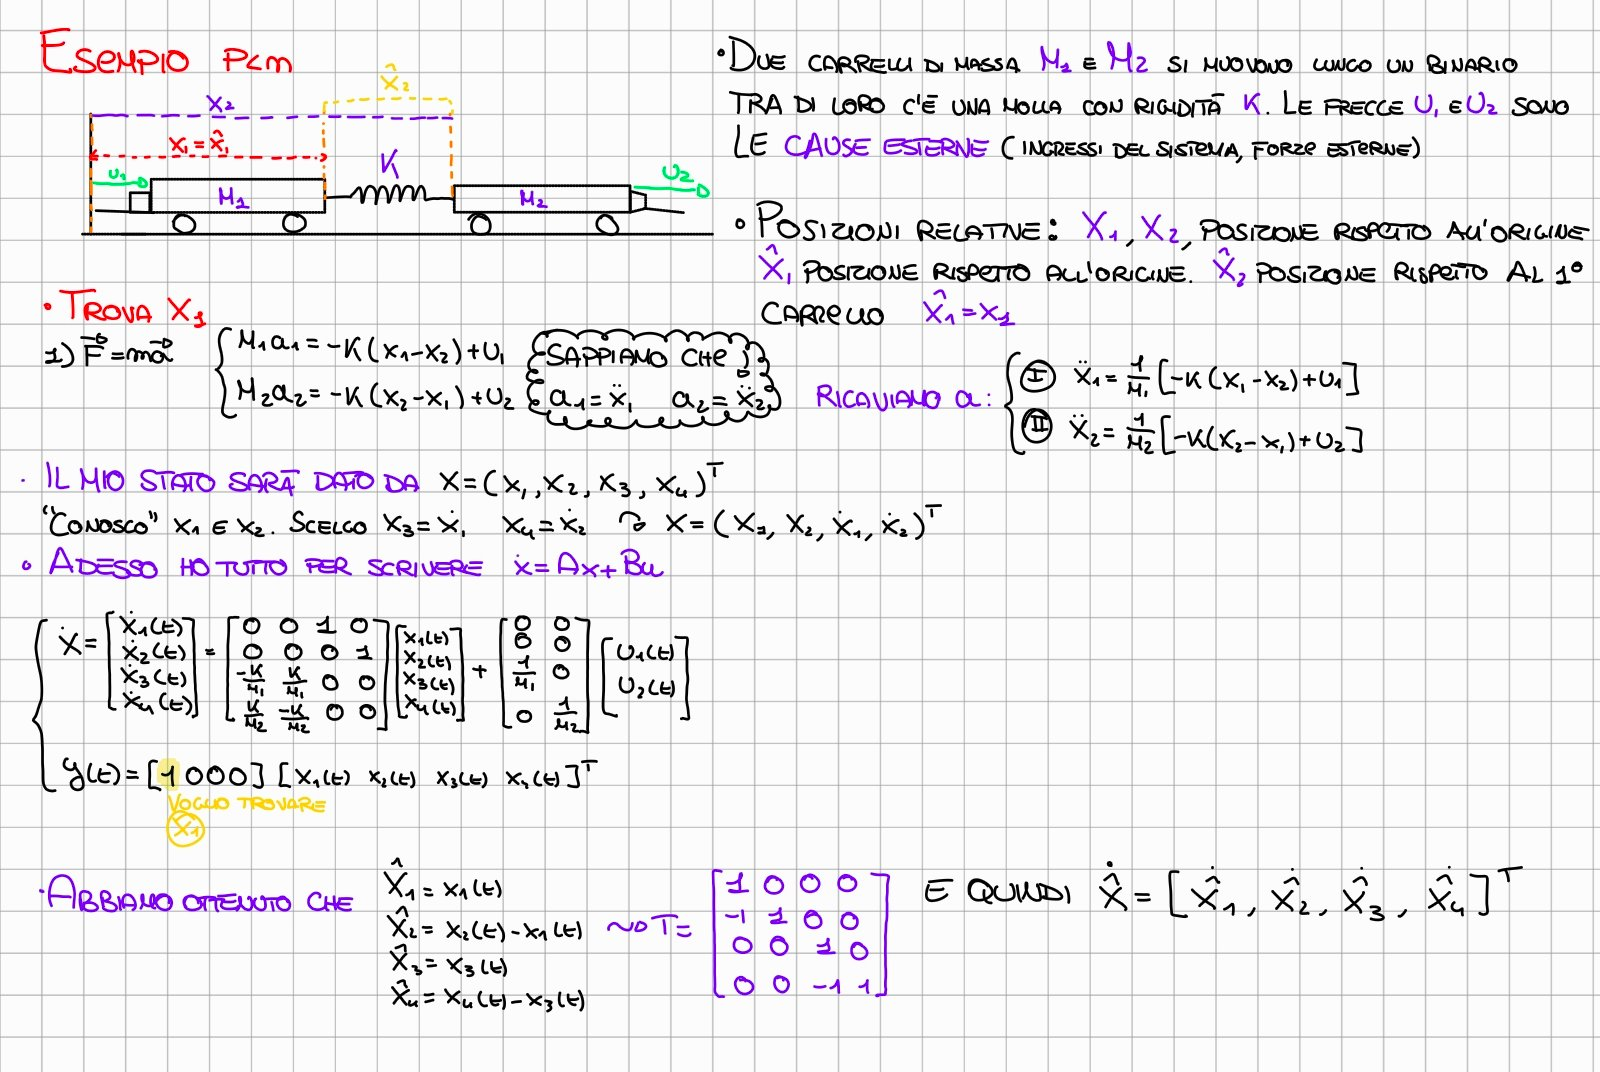
\includegraphics[width=\textwidth]{figura_2.jpg} 
		\caption{Esempio p < n}
		\label{fig:label_immagine}
	\end{figure}
	\subsection{Autovalori e Modi}
	
	Sappiamo che $x(t) = e^{A(t-t_0)}x(t_0)$ è la soluzione di $\dot{x} = Ax$ con $u(t) = 0$ (caso di movimento libero). A seconda che $A$ sia \textbf{diagonalizzabile} o meno distinguiamo due casi.
	
	\subsubsection*{$A$ diagonalizzabile}
	
	Possiamo scegliere $T$ in modo tale che la matrice della dinamica risulti diagonale:
	
	\[
	A = T^{-1} A_D T \qquad 
	A_D = 
	\begin{bmatrix} 
		\lambda_1 & 0 & 0 \\ 
		0 & \ddots & 0 \\ 
		0 & 0 & \lambda_n 
	\end{bmatrix}
	\]
	
	In questo caso il movimento libero ($\hat{x}_l$) risulta:
	
	\[
	\begin{aligned}
		\hat{x}_l(t) &= e^{A_D t}\hat{x}_0 = \sum_{k=0}^{\infty} \frac{(A_D t)^k}{k!} \hat{x}_0 \qquad 
		(A_D)^k = 
		\begin{bmatrix} 
			(\lambda_1)^k & 0 & 0 \\ 
			0 & \ddots & 0 \\ 
			0 & 0 & (\lambda_n)^k 
		\end{bmatrix} 
		\\[10pt]
		&= \text{diag}\left\{ \sum_{k=0}^{\infty} \frac{(\lambda_1 t)^k}{k!}, \sum_{k=0}^{\infty} \frac{(\lambda_2 t)^k}{k!}, \dots, \sum_{k=0}^{\infty} \frac{(\lambda_n t)^k}{k!} \right\} \hat{x}_0 
		\\[10pt]
		&= \text{diag}\{ e^{\lambda_1 t}, e^{\lambda_2 t}, \dots, e^{\lambda_n t} \} \hat{x}_0
	\end{aligned}
	\]
	
	Riportandoci nelle coordinate originali:
	
	\[
	x_l(t) = T^{-1}\hat{x}_l(t) = T^{-1} \underbrace{\text{diag}\{ e^{\lambda_1 t}, e^{\lambda_2 t}, \dots, e^{\lambda_n t} \}}_{\text{Modi}} T x_0
	\]
	
	In generale, gli autovalori $\lambda$ possono essere numeri complessi. Le funzioni del movimento libero sono quindi combinazioni lineari degli esponenziali degli autovalori di $A$, che vengono detti anche \textbf{modi propri} del sistema:
	
	\[
	y_l(t) = C T^{-1} \text{diag}\{ e^{\lambda_1 t}, e^{\lambda_2 t}, \dots, e^{\lambda_n t} \} T x_0
	\]
	
	\vspace{0.5cm}
	
	\subsubsection*{Esempio: Autovalori Complessi Coniugati}
	
	Consideriamo un sistema definito dalle seguenti matrici e calcoliamone gli autovalori (che risultano complessi coniugati):
	\[
	A = \begin{bmatrix} 1 & 1 \\ -1 & 1 \end{bmatrix}, \qquad 
	C = \begin{bmatrix} 1 & 1 \end{bmatrix}, \qquad 
	\lambda_{1,2} = 1 \pm j
	\]
	
	Definiamo la matrice di trasformazione $T_0$ (che contiene gli autovettori) e la sua inversa $T_0^{-1}$:
	\[
	T_0 = \frac{1}{2} \begin{bmatrix} 1 & -j \\ 1 & j \end{bmatrix}, \qquad 
	T_0^{-1} = \begin{bmatrix} 1 & 1 \\ j & -j \end{bmatrix}
	\]
	
	Applicando la trasformazione, verifichiamo la diagonalizzazione di $A$, ottenendo la matrice $\hat{A}$ (che ha gli autovalori sulla diagonale principale):
	\[
	\hat{A} = T_0 A T_0^{-1} = \begin{bmatrix} 1+j & 0 \\ 0 & 1-j \end{bmatrix}
	\]
	
	Ora calcoliamo il \textbf{movimento libero dello stato} $x_l(t)$. 
	Sostituendo i valori nella formula $x_l(t) = T_0^{-1} e^{\hat{A}t} T_0 x_0$ e applicando la formula di Eulero per convertire gli esponenziali complessi in funzioni trigonometriche reali, otteniamo:
	\begin{align*}
		x_l(t) &= \frac{1}{2} \begin{bmatrix} 1 & 1 \\ j & -j \end{bmatrix} \begin{bmatrix} e^{(1+j)t} & 0 \\ 0 & e^{(1-j)t} \end{bmatrix} \begin{bmatrix} 1 & -j \\ 1 & j \end{bmatrix} x_0 \\[10pt]
		x_l(t) &= e^t \begin{bmatrix} \cos(t) & \sin(t) \\ -\sin(t) & \cos(t) \end{bmatrix} x_0
	\end{align*}
	
	Infine, calcoliamo il \textbf{movimento libero dell'uscita} $y_l(t)$, premoltiplicando lo stato per la matrice $C$:
	\begin{align*}
		y_l(t) &= e^t \begin{bmatrix} 1 & 1 \end{bmatrix} \begin{bmatrix} \cos(t) & \sin(t) \\ -\sin(t) & \cos(t) \end{bmatrix} x_0 \\[10pt]
		y_l(t) &= \sqrt{2} e^t \begin{bmatrix} \cos\left(t + \frac{\pi}{4}\right) & \cos\left(t - \frac{\pi}{4}\right) \end{bmatrix} x_0
	\end{align*}
	\subsection{Studio dei segni di \texorpdfstring{$\lambda$}{lambda} e del comportamento dei modi \texorpdfstring{$e^{\lambda t}$}{e\textasciicircum\{lambda t\}}}
	
	Se la parte reale di $\lambda$ è negativa avremo un'esponenziale decrescente, se invece positiva avremo un'esponenziale crescente. Un comportamento ondulatorio è invece dovuto a un $\lambda$ immaginario. Nota bene che il comportamento ondulatorio si combina con l'esponenziale crescente o decrescente.
	
	Riassumiamo il tutto illustrando un quadro sintetico dell'andamento temporale e qualitativo dei modi in dipendenza della posizione nel piano complesso dei corrispondenti autovalori, rappresentati con crocette.
	
	\vspace{0.8cm}
	
\begin{center}
	\begin{tikzpicture}[>=stealth, scale=0.85, every node/.style={scale=0.9}]
		
		% Assi principali (Piano Complesso)
		\draw[->] (-7.5, 0) -- (7.5, 0) node[below] {Re};
		\draw[->] (0, -5.5) -- (0, 5.5) node[right] {Im};
		\node[below right] at (0,0) {0};
		
		% Coordinate dei poli
		\coordinate (P_neg_real) at (-3,0);
		\coordinate (P_pos_real) at (3,0);
		\coordinate (P_origin)   at (0,0);
		\coordinate (P_lhp_top)  at (-2.5,2.5);
		\coordinate (P_lhp_bot)  at (-2.5,-2.5);
		\coordinate (P_rhp_top)  at (2.5,2.5);
		\coordinate (P_rhp_bot)  at (2.5,-2.5);
		\coordinate (P_im_top)   at (0,3);
		\coordinate (P_im_bot)   at (0,-3);
		
		% Disegno delle crocette azzurre per i poli
		\foreach \p in {P_neg_real, P_pos_real, P_origin, P_lhp_top, P_lhp_bot, P_rhp_top, P_rhp_bot, P_im_top, P_im_bot} {
			\draw[cyan, thick] (\p) ++(-0.15,0.15) -- ++(0.3,-0.3);
			\draw[cyan, thick] (\p) ++(-0.15,-0.15) -- ++(0.3,0.3);
		}
		
		% ================= SUBPLOTS =================
		
		% 1. Esponenziale decrescente (Polo Reale Negativo)
		\begin{scope}[shift={(-6.5, 2)}]
			\draw[->, thin] (-0.2, 0) -- (2.2, 0) node[below] {$t$};
			\draw[->, thin] (0, -0.2) -- (0, 2);
			\node[below left] at (0,0) {0};
			\draw[cyan, thick, domain=0:2, samples=50] plot (\x, {1.5*exp(-\x*1.5)});
			\coordinate (SP1_ptr) at (2, -0.2);
		\end{scope}
		\draw[thin, darkgray, shorten >=2mm] (SP1_ptr) -- (P_neg_real);
		
		% 2. Costante a gradino (Polo nell'Origine)
		\begin{scope}[shift={(2, 3)}]
			\draw[->, thin] (-0.2, 0) -- (2.2, 0) node[below] {$t$};
			\draw[->, thin] (0, -0.2) -- (0, 1.5);
			\node[below left] at (0,0) {0};
			\draw[cyan, thick] (0, 1) -- (2, 1);
			\coordinate (SP2_ptr) at (-0.2, -0.2);
		\end{scope}
		\draw[thin, darkgray, shorten >=2mm] (SP2_ptr) -- (P_origin);
		
		% 3. Esponenziale crescente (Polo Reale Positivo)
		\begin{scope}[shift={(4.5, 0.5)}]
			\draw[->, thin] (-0.2, 0) -- (2.2, 0) node[below] {$t$};
			\draw[->, thin] (0, -0.2) -- (0, 2);
			\node[below left] at (0,0) {0};
			\draw[cyan, thick, domain=0:2, samples=50] plot (\x, {0.3*exp(\x*0.9)});
			\coordinate (SP3_ptr) at (-0.2, 0);
		\end{scope}
		\draw[thin, darkgray, shorten >=2mm] (SP3_ptr) -- (P_pos_real);
		
		% 4. Sinusoide smorzata (Poli complessi coniugati LHP)
		\begin{scope}[shift={(-6.5, -3)}]
			\draw[->, thin] (-0.2, 0) -- (2.5, 0) node[below] {$t$};
			\draw[->, thin] (0, -1.2) -- (0, 1.2);
			\node[below left] at (0,0) {0};
			\draw[cyan, thick, domain=0:2.3, samples=100] plot (\x, {1*exp(-\x*0.6)*cos(deg(3*pi*\x))});
			\coordinate (SP4_ptr) at (2.5, 0.2);
		\end{scope}
		\draw[thin, darkgray, shorten >=2mm] (SP4_ptr) -- (P_lhp_bot);
		
		% 5. Sinusoide pura (Poli immaginari puri)
		\begin{scope}[shift={(-3, -5)}]
			\draw[->, thin] (-0.2, 0) -- (2.5, 0) node[below] {$t$};
			\draw[->, thin] (0, -1.2) -- (0, 1.2);
			\node[below left] at (0,0) {0};
			\draw[cyan, thick, domain=0:2.3, samples=100] plot (\x, {1*cos(deg(3*pi*\x))});
			\coordinate (SP5_ptr) at (2.5, 0.2);
		\end{scope}
		\draw[thin, darkgray, shorten >=2mm] (SP5_ptr) -- (P_im_bot);
		
		% 6. Sinusoide divergente (Poli complessi coniugati RHP)
		\begin{scope}[shift={(4, -4)}]
			\draw[->, thin] (-0.2, 0) -- (2.5, 0) node[below] {$t$};
			\draw[->, thin] (0, -1.2) -- (0, 1.2);
			\node[below left] at (0,0) {0};
			\draw[cyan, thick, domain=0:2.3, samples=100] plot (\x, {0.2*exp(\x*0.7)*cos(deg(3*pi*\x))});
			\coordinate (SP6_ptr) at (-0.2, 0);
		\end{scope}
		\draw[thin, darkgray, shorten >=2mm] (SP6_ptr) -- (P_rhp_bot);
		
	\end{tikzpicture}
	\end{center}
	\subsection*{Analisi del grafico: poli nel piano complesso e andamenti temporali}
	
	Il grafico illustra la relazione fondamentale tra la posizione degli autovalori (o ``poli'', indicati con $\lambda$) nel piano complesso e il corrispondente movimento libero del sistema nel dominio del tempo.
	
	\subsubsection*{1. Perché alcune crocette non sono collegate? (I Poli Coniugati)}
	
	Le crocette azzurre rappresentano gli autovalori del sistema. Nei sistemi fisici reali (le cui matrici sono composte da numeri reali), se un autovalore è complesso, esso si presenterà sempre accompagnato dal suo complesso coniugato. In altre parole, si presentano in \textbf{coppie complesse coniugate}. 
	
	Se è presente un polo nel semipiano superiore (ad esempio, $\lambda = -a + j\omega$), vi sarà obbligatoriamente il suo speculare nel semipiano inferiore ($\lambda = -a - j\omega$). Questi due poli lavorano \textit{congiuntamente} per generare un unico movimento oscillatorio reale nel tempo. Per non sovraccaricare il grafico di linee, si collega solo un polo della coppia al relativo andamento temporale, essendo implicito che l'altro polo speculare contribuisca alla medesima dinamica.
	
	\subsubsection*{2. Come leggere la mappa del piano complesso}
	
	Il piano complesso funge da vera e propria ``mappa'' predittiva. Combinando l'informazione sull'asse orizzontale e verticale, è possibile dedurre qualitativamente la stabilità e la forma della risposta del sistema:
	
	\begin{itemize}
		\item \textbf{L'Asse Orizzontale (Asse Reale, $\text{Re}$): Determina la convergenza o la divergenza.}
		\begin{itemize}
			\item \textbf{Semipiano Sinistro ($\text{Re} < 0$):} È la regione della \textbf{stabilità asintotica}. L'esponenziale associato $e^{\text{Re}(\lambda)t}$ decade a zero. Più il polo è posizionato a sinistra, più l'esaurimento del transitorio è rapido.
			\item \textbf{Semipiano Destro ($\text{Re} > 0$):} È la regione dell'\textbf{instabilità}. L'esponenziale cresce divergendo all'infinito col passare del tempo.
			\item \textbf{Nell'origine ($\text{Re} = 0, \text{Im} = 0$):} Corrisponde a un comportamento costante (assimilabile a un gradino). Denota una condizione di stabilità semplice (o marginale).
		\end{itemize}
		
		\vspace{0.3cm}
		
		\item \textbf{L'Asse Verticale (Asse Immaginario, $\text{Im}$): Determina le oscillazioni.}
		\begin{itemize}
			\item \textbf{Sull'asse reale ($\text{Im} = 0$):} L'autovalore è reale puro. La risposta temporale è costituita da soli andamenti esponenziali, privi di qualsiasi oscillazione.
			\item \textbf{Fuori dall'asse reale ($\text{Im} \neq 0$):} La parte immaginaria dà origine a componenti armoniche (seno e coseno). Il sistema presenterà un comportamento oscillatorio. Più le crocette si allontanano verticalmente dall'asse reale, maggiore sarà la pulsazione dell'oscillazione (frequenza più elevata).
			\item \textbf{Sull'asse immaginario ($\text{Re} = 0, \text{Im} \neq 0$):} Generano oscillazioni persistenti e non smorzate. In assenza di parte reale, il sistema oscilla indefinitamente con ampiezza costante (stabilità semplice).
		\end{itemize}
	\end{itemize}
	% --- FINE GRAFICO TIKZ ---
\end{document}
